\documentclass[conference]{IEEEtran}

\usepackage{cite}
\usepackage{amsmath}
\usepackage{graphicx}
\usepackage{booktabs}
\usepackage[T1]{fontenc}
\usepackage[utf8]{inputenc}
\usepackage{url}
\usepackage[hidelinks]{hyperref}

\begin{document}

\title{Are Employees Satisfied With Their Compensation?\\
A Mixed-Methods Research Proposal for Measuring\\
Pay Satisfaction and Perceived Fairness\\
Among Early-Career Technology Professionals}

\author{\IEEEauthorblockN{Md. Rakib Hossain}
\IEEEauthorblockA{Department of Computer Science and Engineering\\
American International University--Bangladesh\\
Dhaka, Bangladesh\\
Email: 000.mdrakibhossain@gmail.com}}

\maketitle

\begin{abstract}
\textbf{Purpose:} This proposal sets out a study to measure how satisfied
early-career technology professionals are with their compensation, and to
identify which factors shape that judgement.
\textbf{Research question:} To what extent are early-career technology
professionals satisfied with their current compensation, and what
attributes explain variation in that satisfaction?
\textbf{Hypothesis:} H\textsubscript{1} --- pay satisfaction is driven less
by absolute salary than by perceived fairness relative to role,
responsibility, and market rate; H\textsubscript{0} --- pay satisfaction
varies only with absolute salary level.
\textbf{Methodology:} A cross-sectional mixed-methods design combines a
structured questionnaire with semi-structured follow-up interviews.
Quantitative responses are summarised descriptively and triangulated
against coded qualitative accounts.
\textbf{Research participants:} Approximately 120 salaried technology
professionals aged 21--30 with up to five years of professional
experience, recruited from software, data, and design roles in Dhaka.
\textbf{Research tools:} A fifteen-item questionnaire adapted from the
Pay Satisfaction Questionnaire, a semi-structured interview guide, and a
structured literature review.
\textbf{Probable result:} A pilot of thirteen respondents returned a mean
satisfaction of 3.38 on a five-point scale, with only 38.5\,\% rating
four or above and the modal response at neutral. The full study is
therefore expected to find predominantly neutral rather than positive
compensation satisfaction, with dissatisfaction concentrated in
perceptions of fairness rather than in salary magnitude.
\textbf{Conclusion and recommendation:} If confirmed, the finding implies
that employers cannot resolve compensation dissatisfaction through pay
increases alone; transparent pay structures and explicit role-to-pay
mapping are likely to matter more. The instrument and analysis plan
described here are offered as a replicable basis for that assessment.
\end{abstract}

\begin{IEEEkeywords}
compensation satisfaction, pay satisfaction, perceived fairness, equity
theory, employee retention, mixed-methods research
\end{IEEEkeywords}

\section{Introduction}

Compensation is the most direct exchange between an employer and an
employee, yet satisfaction with it is not a simple function of amount.
Two people paid identically may evaluate their pay very differently
depending on what they believe they contribute, what they believe others
receive, and what they believe the market rate to be. This gap between
the objective figure and the subjective judgement is what makes
compensation satisfaction worth measuring separately from compensation
itself.

The distinction matters practically. Organisations that treat
dissatisfaction as a pricing problem respond with across-the-board
increases, which are expensive and, if the underlying grievance concerns
fairness rather than magnitude, ineffective. A study that separates the
two allows a more targeted response.

This proposal describes a study designed to make that separation. It
states the research question and hypotheses, specifies the population and
sampling frame, details the three instruments, and reports pilot data
that motivate the design. The pilot is small and its limitations are
stated plainly; it is presented as evidence that the instrument functions
and that the phenomenon is worth studying at scale, not as a finding in
its own right.

\section{Literature Review}

Research on pay satisfaction has consistently treated it as a judgement
of relative rather than absolute standing. Adams's equity theory frames
the employee as comparing a ratio of personal inputs to outcomes against
the corresponding ratio of a referent other; inequity in either direction
produces tension and a motivation to restore balance \cite{adams1963inequity}.
On this account, an employee paid well in absolute terms may still report
dissatisfaction if the comparison is unfavourable.

Herzberg's two-factor theory positions salary as a hygiene factor: its
absence produces dissatisfaction, but its presence does not
proportionally produce satisfaction \cite{herzberg1959motivation}. The
practical implication is asymmetric --- underpayment reliably harms, while
overpayment does not reliably help.

The measurement literature refined the construct further. Heneman and
Schwab demonstrated that pay satisfaction is multidimensional rather than
unitary, and developed the Pay Satisfaction Questionnaire to separate
satisfaction with pay level, benefits, raises, and pay structure and
administration \cite{heneman1985pay}. Treating pay satisfaction as a
single score, as much survey practice still does, therefore risks
collapsing distinct judgements that may move independently.

The largest synthesis of this work is the meta-analysis by Williams,
McDaniel, and Nguyen, covering 240 samples drawn from 203 studies. It
reports that pay level satisfaction correlates with a broad set of
antecedents and outcomes, and that its relationship with actual pay,
while positive, is far from deterministic \cite{williams2006meta}. This
supports the design decision taken here to collect perceptual measures
alongside reported salary rather than to infer satisfaction from salary.

More recent work situates these mechanisms in the technology sector
specifically. Murugan and Philimis find that compensation, recognition,
and work environment jointly determine retention among information
technology employees, with compensation acting alongside rather than
independently of the other two \cite{murugan2025retention}. Their finding
motivates the inclusion of qualitative interviews in the present design,
since a purely numerical instrument cannot capture recognition effects.

Two gaps follow from this review. First, the pay satisfaction literature
is dominated by samples from large Western organisations, leaving
early-career professionals in South Asian technology firms
under-represented. Second, few studies pair a quantitative satisfaction
measure with open qualitative accounts from the same respondents, which
is what would be needed to distinguish a magnitude complaint from a
fairness complaint. This study addresses both.

\section{Research Methodology}

\subsection{Scope and Area}

The study falls within human resource management, specifically the
measurement of compensation satisfaction and perceived pay fairness. It
is empirical and cross-sectional. It does not evaluate compensation
policy, model salary determination, or track satisfaction over time; each
would require a different design.

\subsection{Class and Social Specification}

The target population is salaried early-career technology professionals
employed in Dhaka, Bangladesh. Socially, this group is urban,
university-educated, and employed in the formal private sector. It is
economically heterogeneous despite its educational homogeneity: entry
salaries in the sector span roughly BDT 15{,}000 to BDT 120{,}000 per
month, which is wide enough for equity comparisons to arise within a
single peer group. That internal spread is precisely what makes the
population suitable for testing a relative-comparison hypothesis.

\subsection{Research Participants}

The full study targets approximately 120 participants, a sample size
chosen to support subgroup comparison across role and experience band
while remaining feasible for a single researcher. Participants must be
aged 21--30, hold a completed undergraduate degree, and be in paid
employment with no more than five years of professional experience.

The pilot reported here recruited 13 participants. Their characteristics
are given in Table~\ref{tab:demographics}. All held technology or
technology-adjacent roles --- software engineering, data analysis, and
graphic design --- and all reported an academic background in computer
science or a closely related field.

\begin{table}[htbp]
\caption{Pilot Participant Characteristics ($n=13$)}
\label{tab:demographics}
\centering
\begin{tabular}{@{}ll@{}}
\toprule
\textbf{Attribute} & \textbf{Value} \\
\midrule
Age range & 21--26 years \\
Mean age & 23.5 years \\
Professional experience & 1--5 years (mean 3.0) \\
Highest qualification & BSc 10, MSc 2, other 1 \\
Role: Software Engineer & 6 \\
Role: Data Analyst & 4 \\
Role: Graphic Designer & 1 \\
Role: Other (self-specified) & 2 \\
Reported monthly salary & BDT 15{,}000--120{,}000 \\
\bottomrule
\end{tabular}
\end{table}

\subsection{Research Tools}

Three instruments are used, each addressing a different limitation of the
others.

\textbf{Questionnaire.} A fifteen-item structured questionnaire collects
demographic attributes, professional attributes (experience,
qualifications, publications, projects led, training completed), reported
monthly salary, and a five-point compensation satisfaction rating. The
satisfaction item and its framing are adapted from the Pay Satisfaction
Questionnaire \cite{heneman1985pay}. The instrument is
self-administered and distributed electronically.

\textbf{Semi-structured interview.} A subset of respondents is invited to
a follow-up interview built around one open prompt --- what would make
your compensation feel more fair --- with probes for role comparison,
market awareness, and recognition. The interview exists to recover the
reasoning behind a numerical rating, which the questionnaire cannot
capture. In the pilot this prompt was administered in written form, and
its yield is discussed in Section~IV.

\textbf{Literature review.} A structured review establishes the
theoretical frame, supplies the validated constructs the questionnaire
adapts, and provides the comparison base against which the study's
findings are interpreted.

\subsection{Data Analysis}

Quantitative responses are analysed descriptively: frequency
distribution, mean, median, and mode of the satisfaction rating, reported
overall and disaggregated by role and experience band. Given the intended
sample size, inferential testing is planned only for the full study, and
only where subgroup counts permit.

Qualitative responses are analysed by thematic coding. Open-text answers
are coded inductively, codes are grouped into themes, and theme frequency
is compared against satisfaction ratings from the same respondents. The
comparison is the mechanism by which the hypothesis is tested: if
dissatisfaction is a magnitude problem, low ratings should co-occur with
requests for a specific increase; if it is a fairness problem, low
ratings should co-occur with comparison language.

\subsection{Ethical Considerations}

Participation is voluntary and informed. No names, employer identifiers,
or contact details are collected. Salary data is stored separately from
any identifying attribute, and reported only in aggregate or in bands.
Respondents may withdraw at any point before analysis. Submission
timestamps were removed from the pilot dataset before archiving, since
they were quasi-identifying within a small cohort and served no
analytical purpose.

\section{Exploratory Data Analysis of the Pilot}

Before the pilot responses are used to anticipate anything, they are
profiled for structure, completeness, and internal plausibility. The
exercise is reported here rather than confined to an appendix because one
of its findings changes how the pilot may be read.

\subsection{Completeness}

Fig.~\ref{fig:quality} summarises missingness across the fields used in
analysis. Three patterns emerge. The conditional \emph{other job title}
field is empty for 69.2\,\% of responses, which is expected --- only
respondents who select ``Other'' complete it --- and is reported for
completeness rather than flagged as a defect. Salary is missing for
15.4\,\%: two respondents entered a literal zero, values
treated as non-responses rather than as earnings of zero. Experience and
projects led are each missing one value.

\begin{figure}[htbp]
\centering
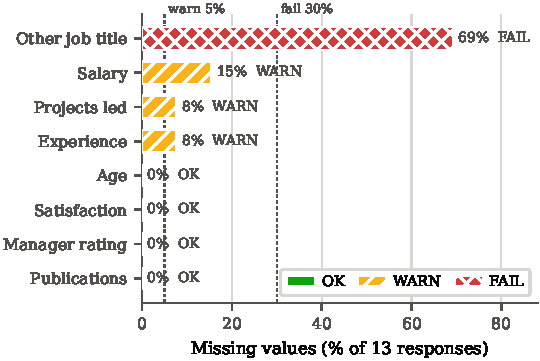
\includegraphics[width=\columnwidth]{eda/fig4_data_quality.pdf}
\caption{Missing values by field. Thresholds at 5\,\% and 30\,\% mark the
warn and fail bands. The 69.2\,\% gap in \emph{other job title} is a
conditional field, not a data-quality failure.}
\label{fig:quality}
\end{figure}

\subsection{Distributions and Outliers}

An interquartile-range screen flags outliers in four fields. Publications
is the most extreme: the distribution is strongly right-skewed
($\text{skew}=1.99$, mean $6.69$, maximum $30$), and the three highest
values --- $10$, $26$, and $30$ --- come from respondents aged 22 to 25 with
four to five years of experience. A publication count of thirty at that
career stage is not credible, and the most likely explanation is that
respondents interpreted the question more broadly than intended. The item
requires rewording before the full study.

Reported salary is similarly distorted. Its standard deviation
(BDT 167{,}276) exceeds its mean (BDT 153{,}182), with a maximum of
BDT 500{,}000 per month against a median of BDT 70{,}000. For the roles
reported, the three highest values are implausible as monthly figures and
may be annual amounts entered in a monthly field.

One further observation concerns the department field. After normalising
case and spelling variants, it collapses to a \emph{single} distinct
value: every respondent reported a computer-science department. The field
therefore has zero variance and can discriminate nothing. This confirms
the homogeneity noted in Section~III-C and is the reason the full study
recruits across firms rather than through one academic network.

\subsection{The Salary--Satisfaction Relationship}

The pilot's most consequential finding concerns the association between
pay and satisfaction, shown in Fig.~\ref{fig:scatter}. Across all eleven
respondents who reported a usable salary, the correlation is moderately
\emph{negative} ($r=-0.58$ Pearson, $\rho=-0.54$ Spearman) --- higher
earners appear less satisfied.

That result does not survive scrutiny. Restricting the calculation to the
eight respondents whose salary is plausible for their stated role
eliminates it entirely ($r=-0.02$). The apparent inverse relationship is
an artefact of three suspect data points, not a property of the
population.

\begin{figure}[htbp]
\centering
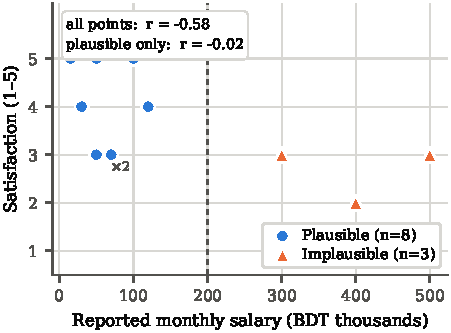
\includegraphics[width=\columnwidth]{eda/fig2_salary_scatter.pdf}
\caption{Reported salary against satisfaction. Triangles mark the three
entries above BDT 200{,}000 per month judged implausible for the stated
role. The correlation across all points ($r=-0.58$) collapses to
$r=-0.02$ once they are excluded. ``$\times 2$'' marks two coincident
respondents.}
\label{fig:scatter}
\end{figure}

The methodological lesson is worth stating plainly, because it would have
been easy to report the headline figure and stop. A correlation computed
over eleven observations can be driven almost entirely by three of them.
Had the negative coefficient been reported without the plausibility
screen, the paper would have claimed an inverse pay--satisfaction
relationship on the strength of three probable data-entry errors.

The screened result still bears on the hypothesis, but through absence
rather than through sign: within this cohort, salary and satisfaction are
essentially \emph{unrelated}. That is consistent with
H\textsubscript{1} --- satisfaction tracking perceived fairness rather than
magnitude --- and inconsistent with H\textsubscript{0}, which requires
satisfaction to rise with pay.

\subsection{What Does Covary With Satisfaction}

Fig.~\ref{fig:corr} gives the Spearman correlation matrix. The strongest
positive correlate of satisfaction is not salary but the manager
performance rating ($\rho=+0.70$), followed by self-rated skill
($\rho=+0.50$). Both are recognition measures rather than pay measures,
which is the association Murugan and Philimis report for information
technology employees \cite{murugan2025retention}.

\begin{figure}[htbp]
\centering
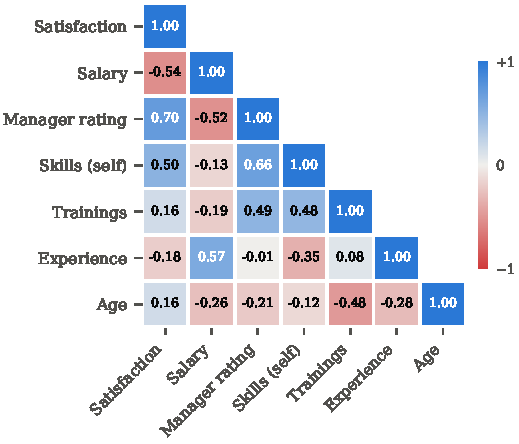
\includegraphics[width=\columnwidth]{eda/fig3_correlation.pdf}
\caption{Spearman rank correlations among pilot variables. The diverging
scale is symmetric about zero with a neutral midpoint; cell values are
printed so the matrix reads without colour.}
\label{fig:corr}
\end{figure}

At $n=13$ none of these coefficients is statistically meaningful, and
none is reported with a $p$-value for that reason. They are recorded as
directions worth testing at scale, not as findings.

\section{Probable Results}

The pilot provides a basis for anticipating the full study's outcome.
Table~\ref{tab:satisfaction} and Fig.~\ref{fig:satisfaction} report the
observed distribution.

\begin{figure}[htbp]
\centering
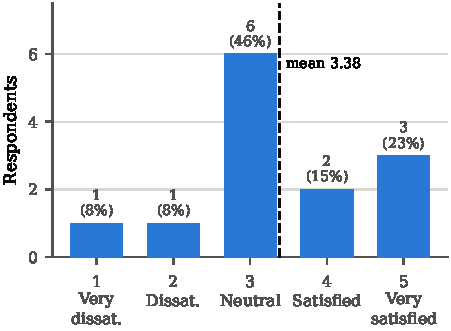
\includegraphics[width=\columnwidth]{eda/fig1_satisfaction.pdf}
\caption{Compensation satisfaction in the pilot ($n=13$). The modal
response is the neutral midpoint; fewer than two respondents in five rate
their compensation at 4 or above.}
\label{fig:satisfaction}
\end{figure}

\begin{table}[htbp]
\caption{Pilot Compensation Satisfaction Distribution ($n=13$)}
\label{tab:satisfaction}
\centering
\begin{tabular}{@{}lcc@{}}
\toprule
\textbf{Rating} & \textbf{Count} & \textbf{Share} \\
\midrule
5 --- Very satisfied & 3 & 23.1\,\% \\
4 --- Satisfied & 2 & 15.4\,\% \\
3 --- Neutral & 6 & 46.2\,\% \\
2 --- Dissatisfied & 1 & 7.7\,\% \\
1 --- Very dissatisfied & 1 & 7.7\,\% \\
\midrule
\textbf{Mean} & \multicolumn{2}{c}{3.38} \\
\textbf{Median / Mode} & \multicolumn{2}{c}{3 / 3} \\
\textbf{Satisfied ($\geq 4$)} & 5 & 38.5\,\% \\
\bottomrule
\end{tabular}
\end{table}

Three patterns are expected to persist at scale.

First, the central tendency is neutral, not positive. Fewer than two in
five pilot respondents rated their compensation satisfaction at four or
above, and the modal response was the midpoint. The full study is
therefore expected to find that early-career technology professionals are
predominantly neutral about their compensation rather than satisfied
with it.

Second, the qualitative responses point to fairness rather than
magnitude. Where respondents elaborated, they described compensation
that should reflect ``role, responsibilities, workload, and market
standard,'' asked for ``fair evaluation,'' and tied increases to
``responsibilities and performance.'' Only one response named a specific
figure. This is the pattern equity theory predicts
\cite{adams1963inequity} and is consistent with salary operating as a
hygiene factor \cite{herzberg1959motivation}. It is the primary reason
H\textsubscript{1} is favoured over H\textsubscript{0}.

Third, satisfaction is not a function of reported salary. As
Section~IV-C established, the screened association is effectively zero,
while the manager rating shows the strongest positive relationship in the
matrix. This is what the meta-analytic evidence would lead one to expect
\cite{williams2006meta}, and it is the observation that most justifies
collecting perceptual data rather than inferring satisfaction from
payroll records.

These are anticipations, not findings. The pilot is too small to
establish any of them.

\section{Limitations}

The pilot has four limitations that constrain what may be claimed from
it, and that the full study is designed to address.

Sample size is the principal constraint. Thirteen responses support
description only. No significance test is reported here because none
would be meaningful at this $n$, and no proportion given above should be
read as an estimate of a population parameter.

Sampling was non-probabilistic and homogeneous. The exploratory analysis
quantified this: after normalisation the department field held one
distinct value across all thirteen responses. The pilot therefore
describes a single narrow cohort and cannot speak to compensation
satisfaction in other sectors, age groups, or educational backgrounds.
The full study widens recruitment across firms rather than through one
academic network, though it remains a convenience sample.

Self-reported measures were unverified, and two proved unreliable.
Salary contained entries inconsistent with the stated role by an order of
magnitude plus two zeros; the full instrument replaces the free-text
field with banded options, reducing both entry error and disclosure
reluctance. Publication counts reached thirty for a respondent with five
years of experience, indicating that the question was read more broadly
than intended; it requires rewording with an explicit definition.

The satisfaction measure was single-item. Since pay satisfaction is
established as multidimensional \cite{heneman1985pay}, a single rating
conflates satisfaction with pay level, raises, benefits, and
administration. The full study replaces it with a multi-item scale
separating those dimensions.

\section{Conclusion and Recommendations}

This proposal has set out a mixed-methods design for measuring
compensation satisfaction among early-career technology professionals,
combining a structured questionnaire, semi-structured interviews, and a
literature review. Pilot evidence from thirteen respondents indicates
predominantly neutral satisfaction, with elaborated complaints
concentrated on fairness rather than on salary magnitude.

Three recommendations follow, each contingent on the full study
confirming the pilot pattern.

For employers, compensation dissatisfaction should not be treated as
solely a pricing problem. If the grievance concerns the relationship
between pay and responsibility rather than the figure itself, an
across-the-board increase is an expensive response to a
mis-diagnosed cause. Publishing role-to-band mappings and the criteria
governing progression addresses the stated concern more directly.

For practitioners designing compensation reviews, the asymmetry between
magnitude and fairness complaints is measurable and should be measured.
Pairing a satisfaction rating with one open question about fairness costs
little and distinguishes the two.

For researchers, the under-representation of South Asian early-career
technology cohorts in the pay satisfaction literature is worth
addressing. The instrument described here is offered as a replicable
starting point, with the caveat that its single-item satisfaction measure
requires replacement by a multidimensional scale before any inferential
claim is attempted.

\section*{Declarations}

\textbf{Data Availability.} The anonymised pilot dataset and the
processing scripts supporting this proposal are available in the
project repository. Submission timestamps were removed prior to
archiving. Individual-level records containing identifying attributes
are not distributed.

\textbf{Ethics.} Pilot participation was voluntary. No names, employer
identifiers, or contact details were collected. As a course-level pilot
conducted without institutional funding, the study did not undergo formal
ethics board review; the full study will be submitted for review before
data collection begins.

\textbf{Author Contributions (CRediT).} Md. Rakib Hossain ---
Conceptualization, Methodology, Investigation, Data Curation, Formal
Analysis, Writing (original draft), Writing (review and editing).

\textbf{Conflict of Interest.} The author declares no competing
interests.

\textbf{Funding.} This research received no external funding.

\bibliographystyle{IEEEtran}
\bibliography{references}

\end{document}
